\documentclass[10pt]{beamer}
\usetheme[] {Feather}
  
%-------------------------------------------------------
% PACKAGES
%-------------------------------------------------------

\usepackage[utf8]{inputenc}
\usepackage[english]{babel}
\usepackage[T1]{fontenc}
\usepackage{helvet}
\usepackage{amsmath}
\usepackage{amssymb}
\usepackage{mathrsfs}
\usepackage{graphicx}
\usepackage{pdfpages}
\usepackage{tikz}
\usepackage{physics}
\usepackage{realboxes}
\usepackage{siunitx}
\usepackage{pifont}
\usepackage{tikz}

\definecolor{cec1d24}{RGB}{236,29,36}
\definecolor{cffffff}{RGB}{255,255,255}
\def\Put(#1,#2)#3{\leavevmode\makebox(0,0){\put(#1,#2){#3}}}


%-------------------------------------------------------
% DEFFINING AND REDEFINING COMMANDS
%-------------------------------------------------------

% colored hyperlinks
\newcommand{\chref}[2]{
  \href{#1}{{\usebeamercolor[bg]{Feather}#2}}
}
\newcommand\blfootnote[1]{%
  \begingroup
  \renewcommand\thefootnote{}\footnote{#1}%
  \addtocounter{footnote}{-1}%
  \endgroup
}
%-------------------------------------------------------
% INFORMATIONS SUR LA PAGE DE TITRE
%-------------------------------------------------------


\title[Characterization of large volume Double Phase Liquid Argon Time Projection chambers in the WA105/ProtoDUNE project]{
\vspace{3cm}
      \textbf{Characterization of large volume Double Phase Liquid Argon Time Projection chambers in the WA105/ProtoDUNE project} \\
}
\author[Philippe COTTE]
{
    Philippe COTTE
}
\date{April 5th 2019}

%-------------------------------------------------------
% CORPS DE LA PRESENTATION
%-------------------------------------------------------

\begin{document}

%-------------------------------------------------------
% PAGE DE TITRE
%-------------------------------------------------------

{\1% % this is the name of the PDF file for the background
    \begin{frame}[plain,noframenumbering] % the plain option removes the header from the title page, noframenumbering removes the numbering of this frame only
        \titlepage % call the title page information from above
    \end{frame}}
    
%    \begin{frame}{Context}{Neutrino oscillations : main questions}
%    	\begin{scriptsize}
%    	\begin{minipage}{0.48\textwidth}
%    			Neutrinos can change flavor through PMNS matrix $\Rightarrow$ they have mass\\
%    			
%	    		 $
%		    		 \left(\begin{matrix}
%		    		 \nu_e \\ \nu_{\mu} \\ \nu_{\tau}
%		    		 \end{matrix}\right) =
%		    		 \left(\begin{matrix}
%		    		 U_{e1} & U_{e2} & \textcolor{red}{U_{e3}} \\
%		    		 \textcolor{red}{U_{\mu 1}} & \textcolor{red}{U_{\mu 2}} & U_{\mu 3}  \\
%		    		 \textcolor{red}{U_{\tau 1}} & \textcolor{red}{U_{\tau 2}} & U_{\tau 3} 
%		    		 \end{matrix}\right)
%		    		 \left(\begin{matrix}
%		    		 \nu_1 \\ \nu_2 \\ \nu_3
%		    		 \end{matrix}\right)
%	    		$\\
%	    		
%	    		Probability to change flavor : \\
%	    		$
%		    		P(\nu_{\mu}\to\nu_e) = $ \\ 
%	    		$
%		    		- 4\sum_{i>j}\Re(U_{\mu i}U_{e i}^*U_{\mu j}^*U_{e j})\sin^2\left(\textcolor{blue}{\Delta m_{ij}^2}\frac{L}{4E}\right) $\\
%	    		$
%		    		 +2\sum_{i>j}\Im(U_{\mu i}U_{e i}^*U_{\mu j}^*U_{e j})\sin\left(\textcolor{blue}{\Delta m_{ij}^2}\frac{L}{2E}\right)
%    		   $ \\
%    		\includegraphics[width=\textwidth]{figures/contexte/numu-nue-vs-L-3flav.png}
%    	\end{minipage}
%    	\hfill
%    	\begin{minipage}{0.48\textwidth}
%    		\begin{itemize}
%    			\item[$\bullet$] $\textcolor{red}{U_{\alpha i}}$ terms contain $e^{i\delta_{CP}}$
%    			\item[$\bullet$] If $\delta_{CP} \ne 0$ and $\pi$: $P(\nu_{\mu}\to\nu_e) \ne P(\overline{\nu}_{\mu}\to\overline{\nu}_e)$
%    		\end{itemize}
%    		$\Rightarrow$ Possible \textcolor{red}{CP violation} in leptonic sector \\ 
%    		$\Rightarrow$ could explain matter-antimatter asymmetry in the universe\\
%	    	
%	    	\begin{itemize}
%	    		\item[$\bullet$]$\textcolor{blue}{\Delta m_{ij}^2} = m_i^2-m_j^2$
%	    		\item[$\bullet$] $\Delta m_{21(sol)}^2\simeq \SI{e-5}{\electronvolt\squared}$
%	    		\item[$\bullet$] $|\Delta m_{31(atm)}^2| \simeq |\Delta m_{32}^2| \simeq \SI{e-3}{\electronvolt\squared}$
%	    	\end{itemize}
%	    	$\Rightarrow$ Unknown \textcolor{blue}{mass hierarchy} : \\
%	    	\includegraphics[width=0.8\textwidth]{figures/contexte/mass_hierarchy.png}\\
%	    	Many BSM theories depend on  \textcolor{blue}{MH}
%	    \end{minipage}
%	\end{scriptsize}
%	    
%    \end{frame}
    
    \begin{frame}{Context}{DU$\nu$E : a longue baseline neutrino oscillation experiment}
    	\begin{scriptsize}
    	\begin{minipage}{0.58\textwidth}
    		The Deep Underground Neutrino Experiment:\\
    		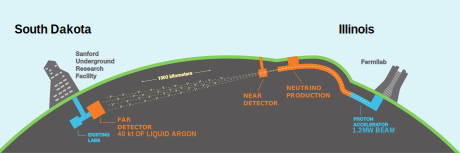
\includegraphics[width=\textwidth]{figures/contexte/dune.jpg}\\
    		
    		1 of the 4 far detector modules:\\
    		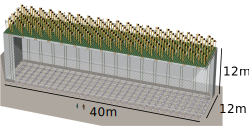
\includegraphics[width=\textwidth]{figures/contexte/dune_module.png}\\
    	\end{minipage}
    	\hfill
    	\begin{minipage}{0.38\textwidth}
    		\begin{itemize}
    			\item[$\bullet$] Neutrino experiment in USA scheduled for 2026.
    			\item[$\bullet$] Will detect $\nu$/$\overline{\nu}$ from Femilab in South Dakota.
    			\item[$\bullet$] Will use \textbf{Liquid Argon Time Projection Chamber}.
    		\end{itemize}
    		\vspace{.3cm}
    		$\Rightarrow$ \textbf{ProtoDU$\nu$E} tests \textbf{two versions} of LArTPC technology at \textbf{tonne scale} at CERN's neutrino platform\\
    		
    		$\Rightarrow$ \textcolor{red}{\textbf{WA105/ProtoDU$\nu$E-DP}} tests the \textcolor{red}{\textbf{Double Phase}} version of LArTPC 
	    \end{minipage}
	\end{scriptsize}
    \end{frame}
    
    \begin{frame}{Context}{DU$\nu$E's detector technology 1 : \textbf{Liquid Argon Time Projection Chamber}}
    	\begin{scriptsize}
    		\begin{minipage}{0.48\textwidth}
    			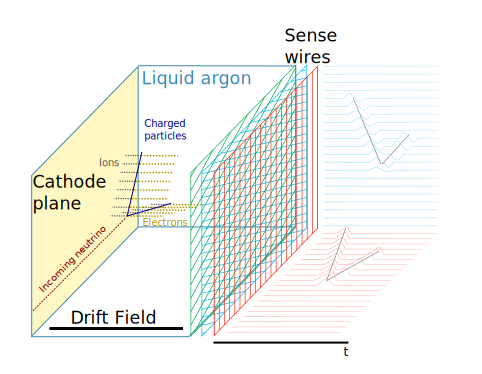
\includegraphics[width=\textwidth]{figures/contexte/lartpc.png}\\
    		\end{minipage}
    		\hfill
    		\begin{minipage}{0.48\textwidth}
    			Advantages of a \textbf{Time Projection Chamber}:    			
    			\begin{itemize}
    				\item[$\bullet$] 3D information.
    				\item[$\bullet$] Big volumes.
    				\item[$\bullet$] Calorimetry.
    				\item[$\bullet$] Particle Identification.
    			\end{itemize}    			
    			Largest LArTPC that detected neutrinos: ICARUS (\SI{600}{\tonne})\\
    			
    			Why Liquid argon?
    			\begin{itemize}
    				\item[$\bullet$] Cheap and abundant.
    				\item[$\bullet$] Scintillates at ionization (used for trigger).
    				\item[$\bullet$] Is inert: does not absorb electrons.
    				\item[$\bullet$] Is dense: ideal for neutrino physics.
    				\item[$\bullet$] Lots of electrons created at ionization.
    			\end{itemize}
    		\end{minipage}
    	\end{scriptsize}
    \end{frame}
    
    \begin{frame}{Context}{DU$\nu$E's detector technology 2 : \textbf{Double Phase LArTPC}}
    	\begin{scriptsize}
    		\begin{minipage}{0.48\textwidth}
    			\includegraphics[width=\textwidth]{figures/contexte/dlartpc.png}\\
    		\end{minipage}
    		\hfill
    		\begin{minipage}{0.48\textwidth}
    			\textbf{Double phase} version: \\\textbf{Amplification} of the signal in gas
    			\begin{itemize}
    				\item[$\bullet$] Allows lower energy threshold.
    				\item[$\bullet$] Allows smaller readout pitch: better 2D resolution.
    				\item[$\bullet$] Allows bigger drift lengths: less dead volumes.
    				\item[$\bullet$] High signal/noise ratio.
    			\end{itemize}    			
    		\end{minipage}
    	\end{scriptsize}
    	\centering
    	DLArTPC is young: biggest one is \SI{250}{\liter}\\
    	\textbf{$\Rightarrow$ needs an extra step of R\&D to reach DU$\nu$E's scale : \textcolor{red}{WA105}}
    \end{frame}
    
    \begin{frame}{Context}{The WA105 project}
		\includegraphics[width=\linewidth]{figures/contexte/wa105}\\
		\begin{scriptsize}
			A demonstrator for the Single Phase is also being tested at CERN's neutrino platform
		\end{scriptsize}
		
    \end{frame}
    
    \begin{frame}{The \texorpdfstring{$6 \times 6 \times \SI{6}{\meter\cubed}$}{666}
    		demonstrator}{Tonne-scale and \si{\meter\squared} readout planes challenges}
    	\begin{scriptsize}
    			\includegraphics[width=0.9\textwidth]{figures/666/666_full.png}\\
    			\vfill
    			\begin{minipage}{0.32\textwidth}
    				\begin{itemize}
    					\item[$\bullet$] Space charge effect?
    					\item[$\bullet$] Purity?
    					\item[$\bullet$] Gain behavior?
    				\end{itemize}
    			\end{minipage}\hfill
    			\begin{minipage}{0.32\textwidth}
    				\begin{itemize}
    					\item[$\bullet$]CRPs planarity?
    					\item[$\bullet$] Max voltages?
    					\item[$\bullet$] Stability?
    				\end{itemize}
	    		\end{minipage}\hfill
	    		\begin{minipage}{0.32\textwidth}
	    			\begin{itemize}
	    				\item[$\bullet$] Track reconstruction?
	    				\item[$\bullet$] Resolution?
	    				\item[$\bullet$] Scalability?
	    			\end{itemize}
	    		\end{minipage}
    	\end{scriptsize} 
    \end{frame}
    
    \begin{frame}{The \texorpdfstring{$6 \times 6 \times \SI{6}{\meter\cubed}$}{666}
    		demonstrator}{The LEM-Anode sandwich}
    	\centering \textbf{Irfu's mission: }Test, characterize and produce  half the LEMs and anodes, for 2 CRPs out of 4.\\\vfill
   		\begin{minipage}{0.48\textwidth}
   			Townsend avalanche:\\
   			\centering  $G = Te^{A\rho d e^{-B\rho d/V}}$\\
   			\begin{scriptsize}
    			\begin{itemize}
    				\item[$\bullet$] $T$: Electric transparency
    				\item[$\bullet$] $A,B$: coefficients, gas dependent.
    				\item[$\bullet$] $d$: amplification length (\SI{1}{\milli\meter}).
    				\item[$\bullet$] $V$: amplification voltage (\SI{3.5}{\kilo\volt}).
    				\item[$\bullet$] $\rho$: gas density.
    			\end{itemize}
    		\end{scriptsize} 
   			\vfill
			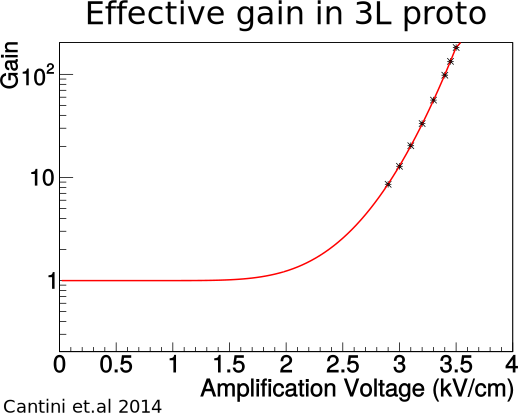
\includegraphics[width=0.9\textwidth]{figures/666/3L_gain.png}
   		\end{minipage}\hfill
   		\begin{minipage}{0.48\textwidth}
   			\includegraphics[width=0.9\textwidth]{figures/666/lem_anode.png}
   		\end{minipage}
    \end{frame}
    
    \begin{frame}{The \texorpdfstring{$6 \times 6 \times \SI{6}{\meter\cubed}$}{666}
    		 demonstrator}{Study of LEM's dead zones}
   		\begin{scriptsize}
    		\begin{minipage}{0.38\textwidth}
    			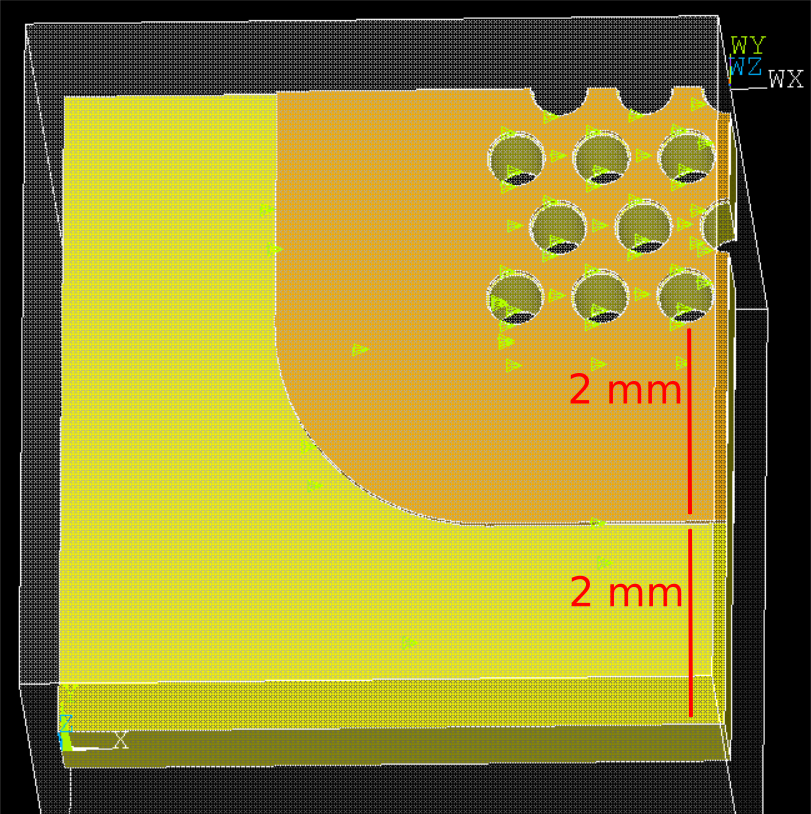
\includegraphics[width=0.8\textwidth]{figures/666/corner_annotations.png}
    			\vspace{0.5cm}\\
    				Dead zones = zones without holes:
    				\begin{itemize}
    					\item[$\bullet$] LEM's borders.
    					\item[$\bullet$] screw holes.
    					\item[$\bullet$] High voltages connectors.
    				\end{itemize}
    				$\Rightarrow$ Impact on collected charge?\\
    				$\Rightarrow$ Impact on charge resolution?\\
    				
    				Use \textbf{ANSYS} to simulate field map through the CRP.\\
    				Simulate drift of electrons in the map with \textbf{GarField}.\\
    		\end{minipage}
    		\begin{minipage}{0.58\textwidth}
    			\centering
    			\includegraphics[width=0.6\textwidth]{figures/666/drift_example.png}\\
    			\vspace{0.5cm} \hspace{0.1cm}
    			\begin{minipage}{0.48\textwidth}
    				\centering
    				LEM's efficiency map\\
    				\includegraphics[width=\textwidth]{figures/666/eff_map.png}
    			\end{minipage}\hfill
    			\begin{minipage}{0.48\textwidth}
    				\centering
    				Impact on reconstructed energy\\
    				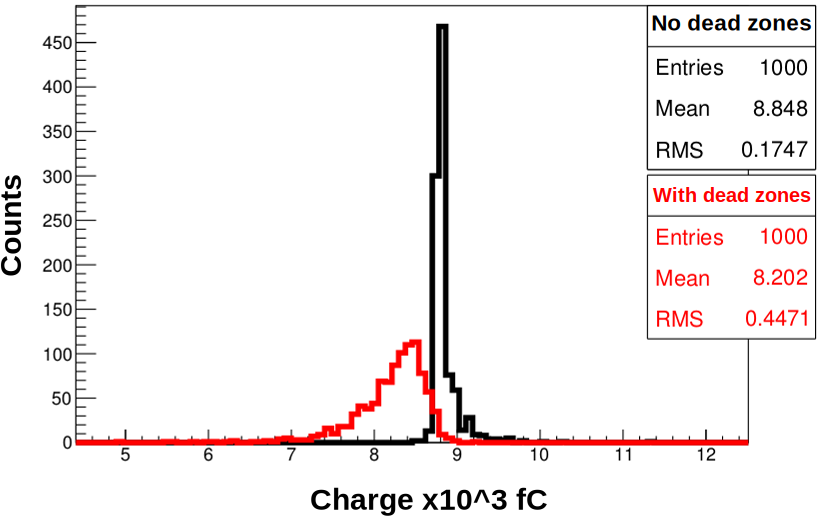
\includegraphics[width=\textwidth]{figures/666/electron.png}
    			\end{minipage}
    		\end{minipage}
    	\end{scriptsize} 
    \end{frame}
    
    \begin{frame}{The \texorpdfstring{$6 \times 6 \times \SI{6}{\meter\cubed}$}{666} demonstrator}{LEM tests in high pressure chamber at Saclay : High voltage}
    	\begin{scriptsize}
    		\begin{center}\textbf{Test LEMs in DLArTPC density conditions : Maximum High Voltage}\end{center}
    		\begin{columns}
		    	\begin{column}{0.5\textwidth}
		    		\includegraphics[height=3.7cm]{figures/666/gamelle.jpg}\\
		    		\begin{itemize}
		    			\item[$\bullet$] High Pressure chamber: Filled with gas argon.
		    			\item[$\bullet$] No cryogenic system: \textcolor{red}{room temperature}.
		    		\end{itemize}
		    	\end{column}\hfill
		    	\begin{column}{0.5\textwidth}
		    		\includegraphics[height=3.7cm]{figures/666/6lems_gamelle.jpg}\\
		    		\begin{itemize}
		    			\item[$\bullet$] To get DLArTPC density: \textcolor{red}{\SI{3.3}{\bar}}.
		    			\item[$\bullet$] Stack of 6-9 LEMs.
		    			\item[$\bullet$] Tested more than 70 LEMs.
		    		\end{itemize}
		    	\end{column}
		    \end{columns}
	    \end{scriptsize} 
    \end{frame}
    
    \begin{frame}{The \texorpdfstring{$6 \times 6 \times \SI{6}{\meter\cubed}$}{666} demonstrator}{LEM tests in high pressure chamber at Saclay : High voltage}
    	\begin{scriptsize}
    		\begin{center}\textbf{Test LEMs in DLArTPC density conditions : Maximum High Voltage}\end{center}
    		\begin{columns}
	    		\begin{column}{0.48\textwidth}
	    			\centering CFR-34 at 33--\SI{35}{\kilo\volt\per\centi\meter}
	    			\includegraphics[height=3.5cm]{figures/666/sparks_34.png}
	    		\end{column}\hfill
	    		\begin{column}{0.48\textwidth}
	    			\centering CFR-35 at \SI{35}{\kilo\volt\per\centi\meter}
	    			\centering 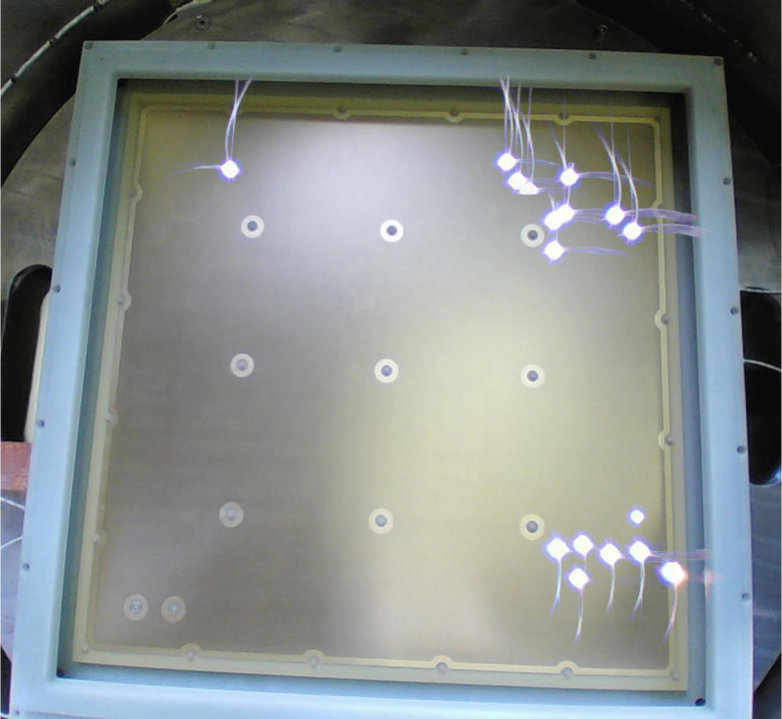
\includegraphics[height=3.5cm]{figures/666/sparks_35.png}
	    		\end{column}
	    	\end{columns}\vfill
	    	\begin{columns}
	    		\begin{column}{0.48\textwidth}
	    			\begin{itemize}
	    				\item[$\bullet$] Initial design (left) could not hold more than \SI{32}{\kilo\volt\per\centi\meter}.
	    				\item[$\bullet$] Sparks mostly on border and corner.
	    			\end{itemize}
	    			$\Rightarrow$ Create new design (right) with larger borders.\\
	    			$\Rightarrow$ \# of sparks reduced by one order of magnitude.
	    		\end{column}\hfill
	    		\begin{column}{0.48\textwidth}
	    			\begin{minipage}{0.48\textwidth}
	    				\centering CFR-34
	    				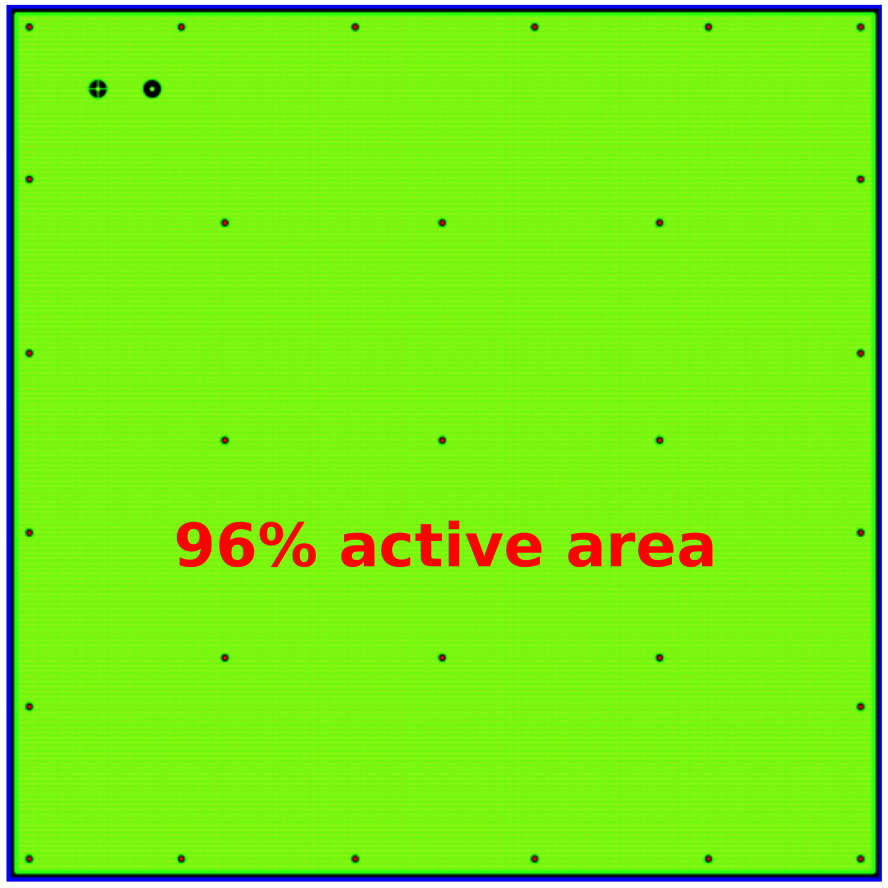
\includegraphics[width=\textwidth]{figures/666/CFR-34.png}
	    			\end{minipage}\hfill
	    			\begin{minipage}{0.48\textwidth}
	    				\centering CFR-35
	    				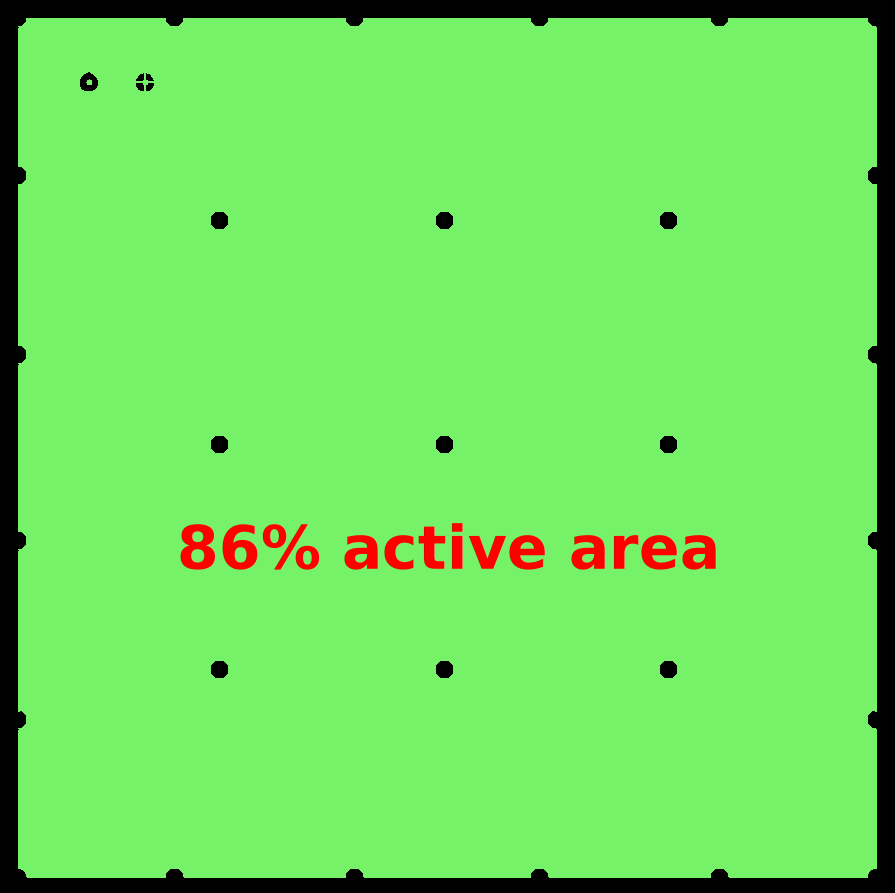
\includegraphics[width=\textwidth]{figures/666/CFR-35.png}
	    			\end{minipage}
	    		\end{column}
	    	\end{columns}
    	\end{scriptsize} 
    \end{frame}
    
    \begin{frame}{The \texorpdfstring{$6 \times 6 \times \SI{6}{\meter\cubed}$}{666} demonstrator}{LEM tests in high pressure chamber at Saclay : gain measurements}
    	\begin{scriptsize}
    		\begin{center}\textbf{Test LEMs in DLArTPC density conditions : Gain}\end{center}
    		\begin{columns}
    			\begin{column}{0.42\textwidth}
    				\centering 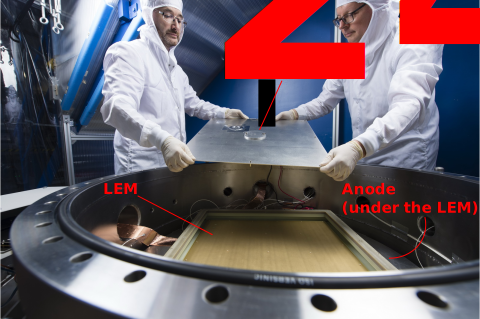
\includegraphics[width=\textwidth]{figures/666/gamelle_source.png}
    			\end{column}\hfill
    			\begin{column}{0.58\textwidth}
    				\centering \includegraphics[width=\textwidth]{figures/666/gain.png}
    			\end{column}
    		\end{columns}\vfill
    		\begin{columns}
    			\begin{column}{0.38\textwidth}
    				\begin{itemize}
    					\item[$\bullet$] 1 LEM-anode sandwich.
    					\item[$\bullet$] $^{241}$Am source.
    				\end{itemize}
    			\end{column}\hfill
    			\begin{column}{0.58\textwidth}
    				\begin{itemize}
    					\item[$\bullet$] At same voltage, all designs have $\sim$ same gain.
    					\item[$\bullet$] \textcolor{red}{Performance resides in maximum high voltage.}
    				\end{itemize}
    			\end{column}
    		\end{columns}
    		\vfill
    		\textbf{$\Rightarrow$ Use CFR-35 for $\mathbf{6 \boldsymbol{\times} 6 \boldsymbol{\times} \SI[detect-weight]{6}{\meter\cubed}}$}.\\
    		\textbf{Note:} Not sure about absolute gain value. Based on 3L measurements, CFR-35 should reach gain of $\sim$200.
    	\end{scriptsize}
    \end{frame}
    
    \begin{frame}{The \texorpdfstring{$6 \times 6 \times \SI{6}{\meter\cubed}$}{666} demonstrator}{LEM thickness measurements}
    	\begin{scriptsize}
    		\begin{columns}
    			\begin{column}{0.48\textwidth}
    				Townsend avalanche:\\
    				\begin{center}
	    				$G = e^{A\rho \textcolor{red}{d} e^{-B\rho \textcolor{red}{d}/V}}$\\
    				\end{center}
    				$\textcolor{red}{d}$: amplification length, i.e \textcolor{red}{LEM thickness}.\\
    				$\Rightarrow$ Exponential impact on gain.\\
    				$\Rightarrow$ Need to know thickness fluctuation in our LEMs to predict \textcolor{red}{gain fluctuations}.\\
    				\vfill
    				\centering \includegraphics[height=0.5\textheight]{figures/666/CCI.png}\\\vfill
	    		\end{column}
	    		\hfill
	    		\begin{column}{0.48\textwidth}
	    			\begin{itemize}
	    				\item[$\bullet$] Use Confocal Chromatic Imaging.
	    				\item[$\bullet$] Measure thickness of the 72 LEMs of the $6 \times 6 \times \SI{6}{\meter\cubed}$.
	    				\item[$\bullet$] Created a Python script to analyze the results.
	    				\item[$\bullet$] Predict gain fluctuations at different amplification voltages.
	    			\end{itemize}
	    			\centering 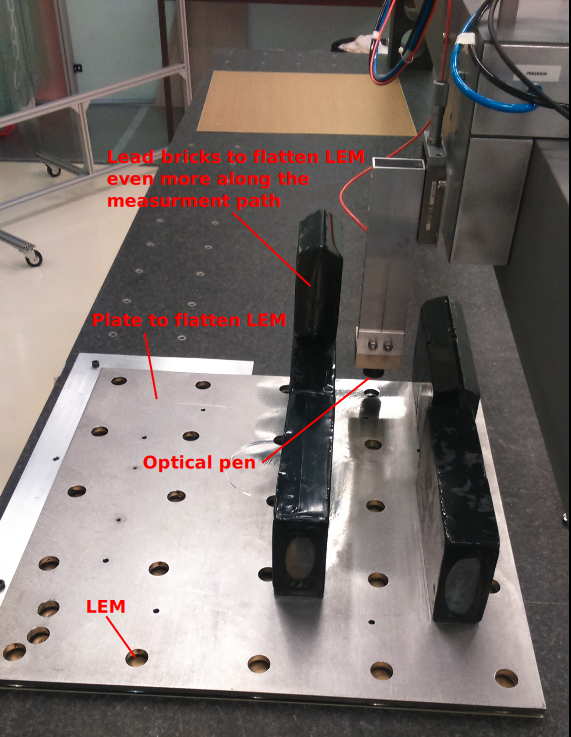
\includegraphics[height=0.5\textheight]{figures/666/plate_and_bricks.png}
	    		\end{column}
	   		\end{columns}
    	\end{scriptsize}
    \end{frame}
    
    \begin{frame}{The \texorpdfstring{$6 \times 6 \times \SI{6}{\meter\cubed}$}{666} demonstrator}{LEM thickness measurements}
    	\begin{scriptsize}
    		\begin{columns}
    			\begin{column}{0.48\textwidth}
    				\centering
    				Thickness distribution in one measurement hole\\
    				
    				 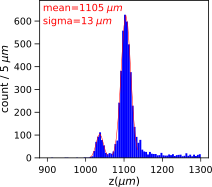
\includegraphics[width=0.6\textwidth]{figures/666/distri_1_trou_lem.png}\\
    				\vfill
    				\centering
    				Mean thickness in all measurement holes \\(36 LEMs)\\
    				
    				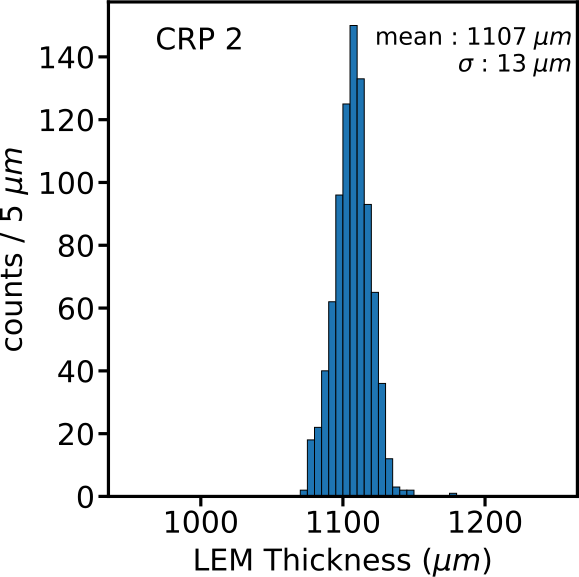
\includegraphics[width=0.6\textwidth]{figures/666/LEM_sum_all_histo_CERN.png}
    			\end{column}
    			\hfill
    			\begin{column}{0.48\textwidth}
    				\centering
    				Mean thickness in 24 measurement holes\\(1 LEM)\\
    				
    				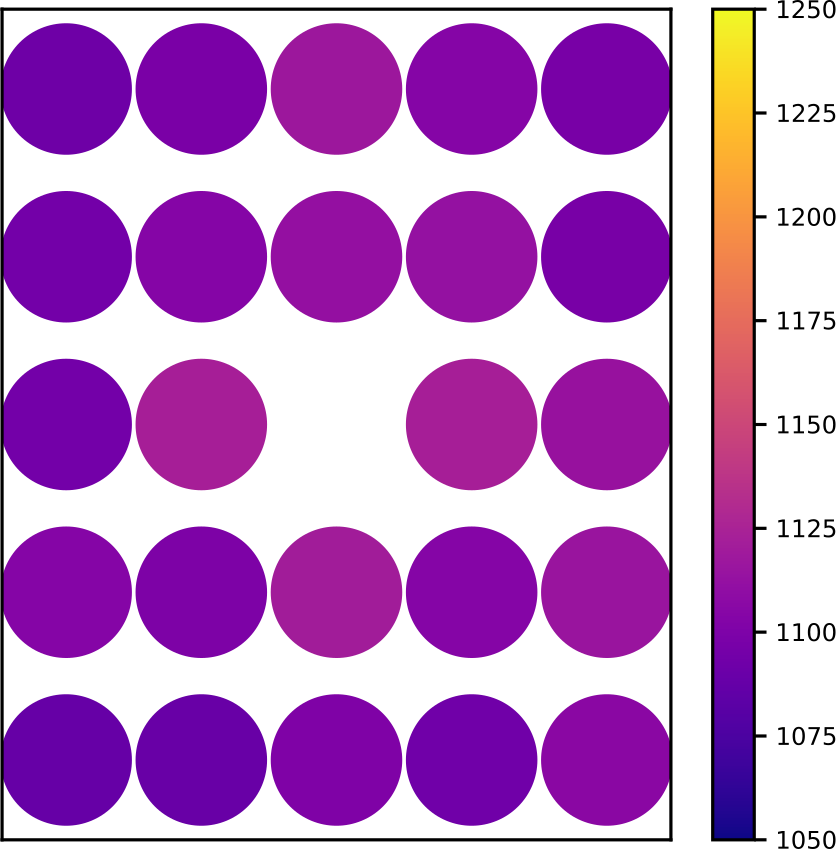
\includegraphics[width=0.6\textwidth]{figures/666/2D_LEM_thickness_distri.png}\\
    				\vfill
    				\centering
    				Expected gain at $d=1107\pm\SI{13}{\micro\meter}$\\
    				\textcolor{red}{$\sim 20\%$ variations at \SI{3.5}{\kilo\volt}}\\
    				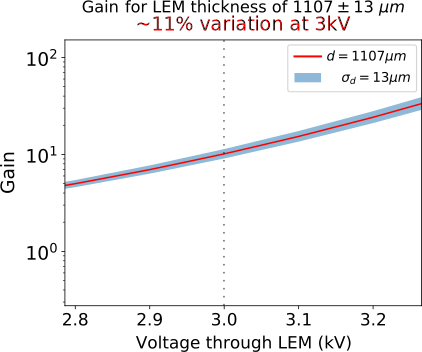
\includegraphics[width=0.6\textwidth]{figures/666/measured_gain_fluctuations.png}
    			\end{column}
    		\end{columns}
    	\end{scriptsize}
    \end{frame}
    
%    \begin{frame}{The \texorpdfstring{$6 \times 6 \times \SI{6}{\meter\cubed}$}{666} demonstrator}{Mounting the CRPs at CERN}
%    	\centering One CRP fully assembled at CERN\\
%    	\vfill
%    		\includegraphics[width=\textwidth]{figures/666/crp_top_bottom.png}
%    \end{frame}
{
	\usebackgroundtemplate{\includegraphics[width=\paperwidth]{figures/666/crp_top_bottom.png}}
	\begin{frame}[plain]
		
	\end{frame}
}
    
    \begin{frame}{The \texorpdfstring{$6 \times 6 \times \SI{6}{\meter\cubed}$}{666} demonstrator}{Full CRP high voltage  tests in cold box}
   		\begin{columns}
   			\begin{column}{0.35\textwidth}
   				\includegraphics[width=\textwidth]{figures/666/crp_inserting_coldbox.png}\\
   				\begin{scriptsize}
   					\begin{itemize}
   						\item[$\bullet$] Maximum High voltage? (LEM and extraction grid)
   						\item[$\bullet$] Stability? (sparks per hour)
   						\item[$\bullet$] Planarity?
   					\end{itemize}
   				\end{scriptsize}
    		\end{column}
    		\begin{column}{0.65\textwidth}
    			\begin{scriptsize}
	    			\textbf{Test the CRPs in real dual-phase conditions in a cold box}
	    		\end{scriptsize}
    			\begin{tiny}
    				\begin{table}[]
    					\begin{scriptsize}
    						\centering CRP 1
    					\end{scriptsize}
    					\begin{tabular}{|l|l|l|l|l|l|l|}
    						\hline
    						\multicolumn{1}{|c|}{\textbf{$\mathbf{V_{top}}$}} & \multicolumn{1}{c|}{\textbf{$\mathbf{V_{bot}}$}} & \multicolumn{1}{c|}{\textbf{$\mathbf{E_{LEM}}$}} & \multicolumn{1}{c|}{\textbf{Time (h)}} & \multicolumn{1}{c|}{\textbf{Sparks/h}} & \multicolumn{1}{c|}{\textbf{$\mathbf{P_{atm}}$}} & \multicolumn{1}{c|}{\textbf{$\mathbf{G_{eff}}$}} \\ \hline
    						0.25 & 3.35 & 31.0 & 12 & 1.3 & 968--972 & \textcolor{green}{20} \\
    						0.50 & 3.55-3.60 & 30.5-31.0 & 13 & 1.3 & 962-966 & \textcolor{green}{24-31} \\
    						0.75 & 3.70 & 29.5 & 42 & 0.6 & 943-953 & \textcolor{green}{20} \\
    						1.00 & 3.80 & 28.0 & 18 & 2 trips & 970-976 & 9 \\
    						1.00 & 3.85 & 28.5 & 12 & 3 trips & 936-947 & 15 \\ \hline
    					\end{tabular}
    				\end{table}
    				\begin{table}[]
    					\begin{scriptsize}
    						\centering CRP 1
    					\end{scriptsize}
    					\begin{tabular}{|l|l|l|l|l|l|l|}
    						\hline
    						\multicolumn{1}{|c|}{\textbf{$\mathbf{V_{top}}$}} & \multicolumn{1}{c|}{\textbf{$\mathbf{V_{bot}}$}} & \multicolumn{1}{c|}{\textbf{$\mathbf{E_{LEM}}$}} & \multicolumn{1}{c|}{\textbf{Time (h)}} & \multicolumn{1}{c|}{\textbf{Sparks/h}} & \multicolumn{1}{c|}{\textbf{$\mathbf{P_{atm}}$}} & \multicolumn{1}{c|}{\textbf{$\mathbf{G_{eff}}$}} \\ \hline
    						0.10 & 3.15-3.20 & 30.5-31.0 & 17 & 0.8 & 969--973 & 9-11 \\
    						0.25 & 3.34 & 30.9 & 16 & 1.3 & 968-970 & 19 \\
    						0.50 & 3.55 & 30.5 & 11 & 0.9 & 957-965 & \textcolor{green}{24} \\
    						0.50 & 3.555 & 30.55 & 42 & 0.5 & 962-964 & \textcolor{green}{25} \\ \hline
    					\end{tabular}
    				\end{table}
    			\end{tiny}
    		\end{column}
    	\end{columns}
    	\vfill
    	\begin{scriptsize}
	    	$\Rightarrow$ Estimated stable gain: $\sim20$.\\
	    	$\Rightarrow$ 1 spark per hour per CRP: ok for DU$\nu$E.
	    \end{scriptsize}
	    \end{frame}
       
       \begin{frame}{The \texorpdfstring{$6 \times 6 \times \SI{6}{\meter\cubed}$}{666} demonstrator}{After cold box tests: carbonisation of corners}
	       	\begin{scriptsize}
	       		\begin{columns}
	       			\begin{column}{0.4\textwidth}
	       				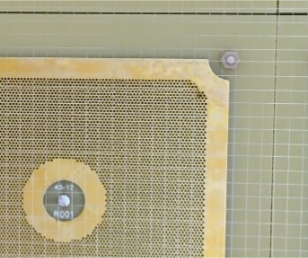
\includegraphics[width=\textwidth]{figures/666/carbonisation.png}\\
	       				\vfill
	       				\begin{itemize}
	       					\item[$\bullet$] Corner of some LEMs got carbonised due to too many sparks\\
	       					(can be cleaned with permanganate)
	       				\end{itemize}
	       			\end{column}
	       			\hfill
	       			\begin{column}{0.6\textwidth}
	       				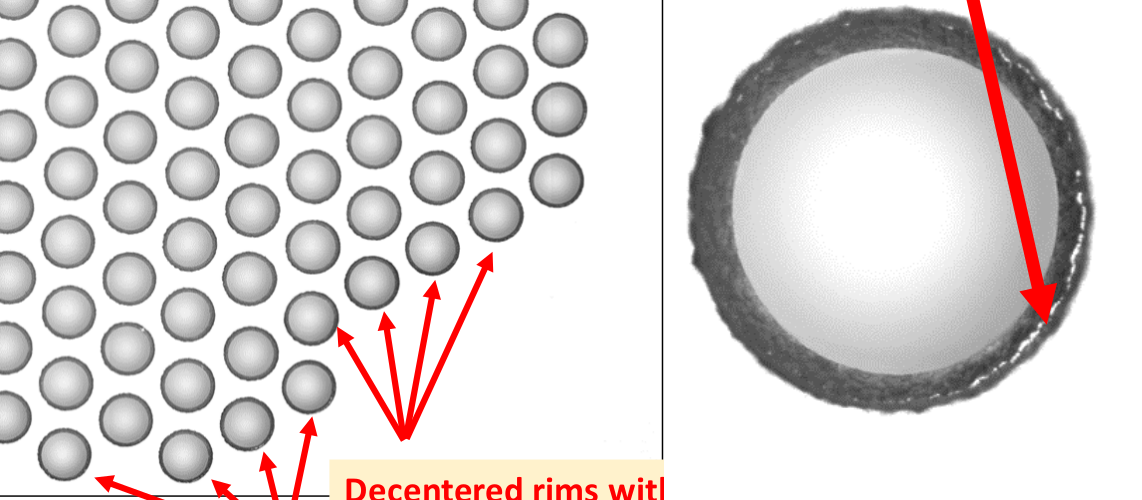
\includegraphics[width=\textwidth]{figures/666/decentered_rims.png}\\
	       				\vfill
	       				\begin{itemize}
	       					\item[$\bullet$] Visual inspection : some RIMs are decentered
	       					\item[$\bullet$] Most likely a problem with chemical etching
	       					\item[$\bullet$] New technique developed at CERN by Rui De Oliveira
	       				\end{itemize}
	       				$\Rightarrow$ Under measurement
	       			\end{column}
	       		\end{columns}
	       	\end{scriptsize}
       \end{frame}
       {
       	\usebackgroundtemplate{\includegraphics[width=\paperwidth]{figures/666/fisheye.png}}
       \begin{frame}[plain]
       	
       \end{frame}
	    }
	    
    \begin{frame}{The \texorpdfstring{$3 \times 1 \times \SI{1}{\meter\cubed}$}{311} prototype}{Goals}
    	\begin{scriptsize}
    		\includegraphics[width=0.48\textwidth]{figures/311/311_2.png}\hfill
    		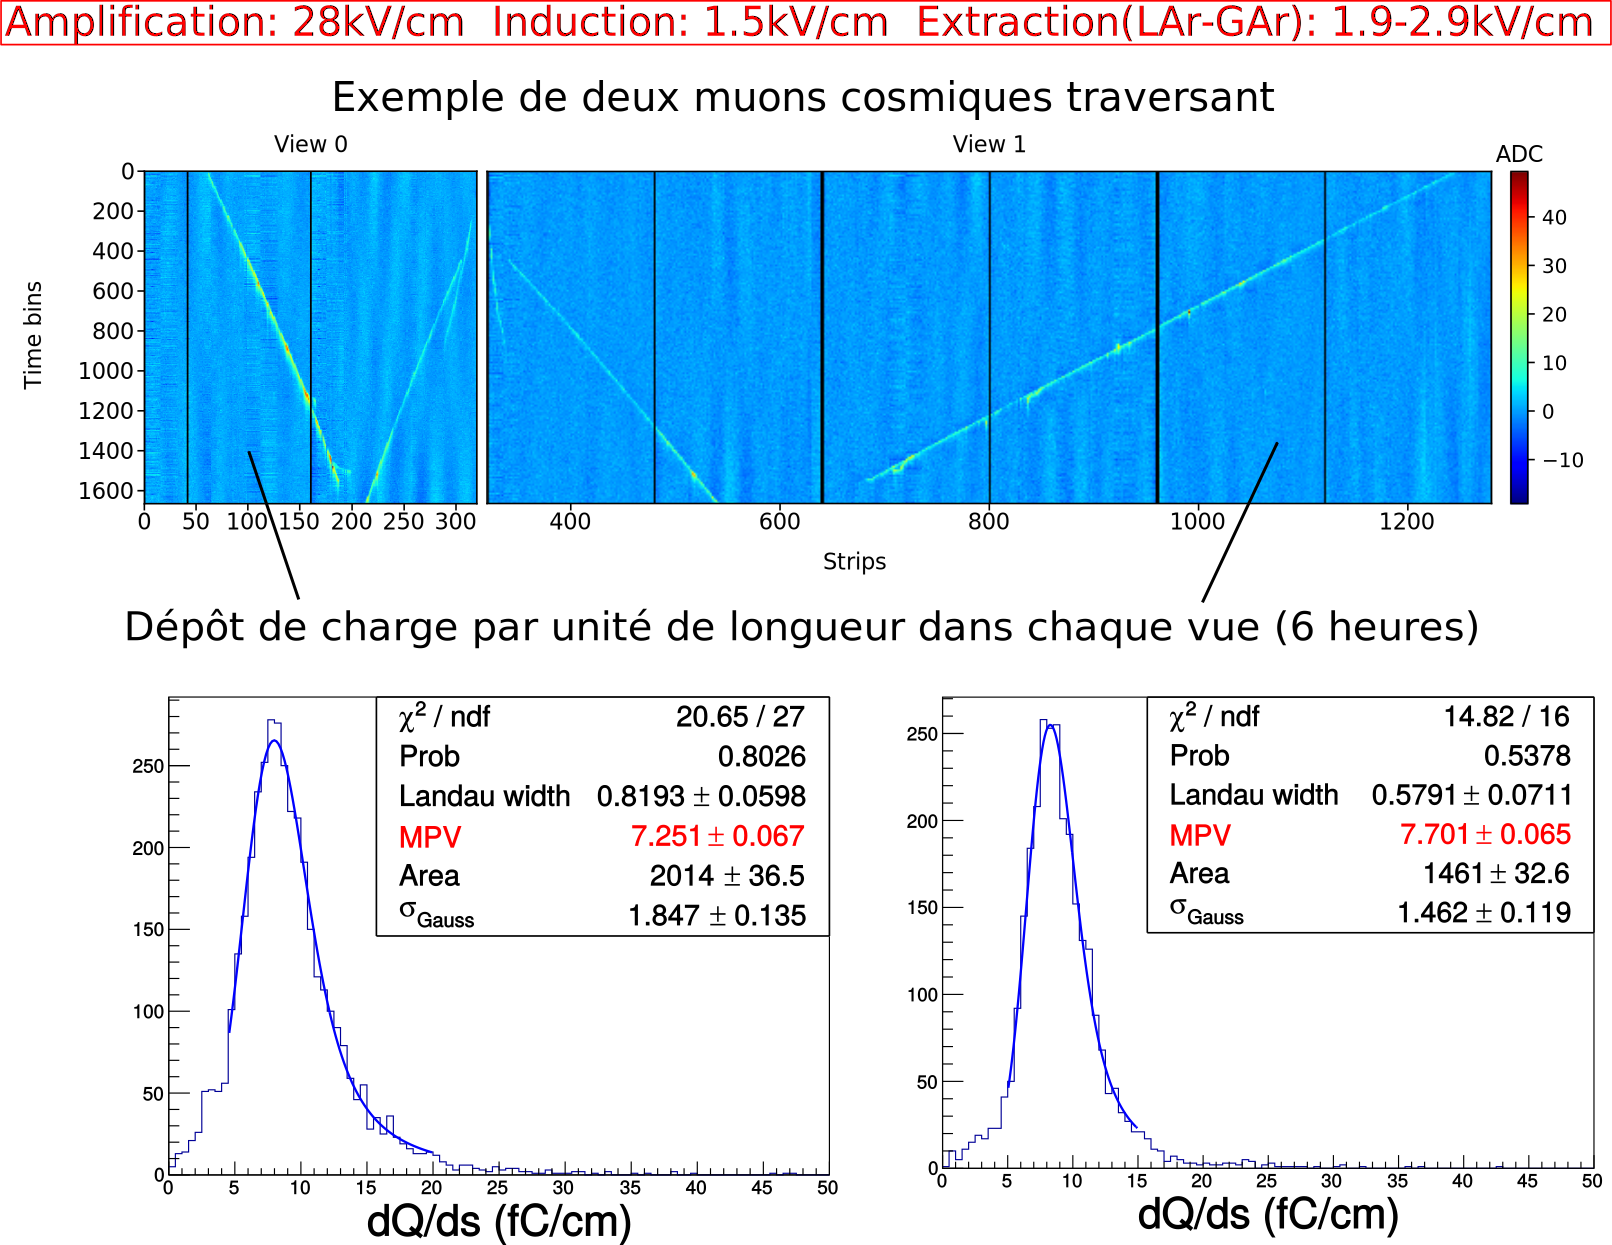
\includegraphics[width=0.45\textwidth]{figures/311/run840.png}\\
    		\vfill
    		\begin{columns}
    			\begin{column}{0.48\textwidth}
    				\textbf{Goal:} Demonstrate the ability of DLArTPC to operate at large volumes and readout surfaces
    				\begin{itemize}
    					\item[$\bullet$] Gain vs Amplification
    					\item[$\bullet$] Charging up
    					\item[$\bullet$] Purity
    					\item[$\bullet$] Reconstruction abilities
    					\item[$\bullet$] Limitations?
    				\end{itemize}
    			\end{column}\hfill
    			\begin{column}{0.48\textwidth}
    				\textbf{Difficulties:} 
    				\begin{itemize}
    					\item[$\bullet$] Loose grid wire provoked discharges: could not operate on long periods
    					\item[$\bullet$] Grid wires not tight enough\\$\Rightarrow$ Vertical displacement\\$\Rightarrow$ Limitation on grid voltage\\$\Rightarrow$ Limitation on LEM voltages
    					\item[$\bullet$] LEM could not hold more than 31kV/cm (CFR-34)
    				\end{itemize}
    				\textcolor{red}{$\Rightarrow$ Solved in the $6 \times 6 \times \SI{6}{\meter\cubed}$}
    			\end{column}
    		\end{columns}
	    \end{scriptsize}
    \end{frame}
    
    
    \begin{frame}{The \texorpdfstring{$3 \times 1 \times \SI{1}{\meter\cubed}$}{311} prototype}{Charging up}
    	\begin{scriptsize}
    		\begin{columns}
    			\begin{column}{0.45\textwidth}
    				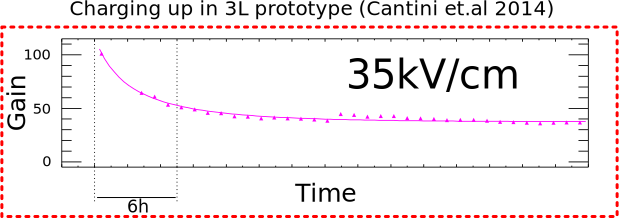
\includegraphics[width=\textwidth]{figures/311/3L_charging_up.png}\\
    				\vfill
    				\begin{itemize}
    					\item[$\bullet$] \textbf{From 3L}: Higher field $\Rightarrow$ quicker charging up.
    					\item[$\bullet$] \textbf{We expect}:
    					\begin{itemize}
    						\begin{scriptsize}
    							\item bigger drift lengths $\Rightarrow$ quicker charging up.
    							\item Bigger surface $\Rightarrow$ no impact
    						\end{scriptsize}
    					\end{itemize}
    					\item[$\bullet$] 3L: 50\% decrease in \SI{6}{\hour}. 
    					\item[$\bullet$] Extrapolating to \SI{28}{\kilo\volt\per\centi\meter}: \textcolor{red}{$\sim$20\% decrease}.
    					\item[$\bullet$]  $3 \times 1 \times \SI{1}{\meter\cubed}$: $\sim$\textcolor{red}{4\% decrease}.
    				\end{itemize}
    			\end{column}\hfill
    			\begin{column}{0.55\textwidth}
    				\centering 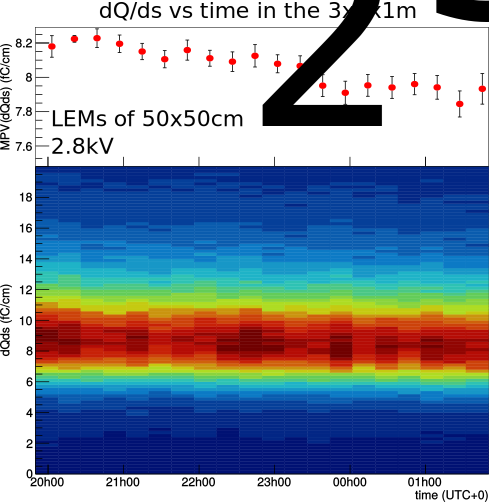
\includegraphics[width=\textwidth]{figures/311/311_charging_up.png}\\
    				\vfill
    			\end{column}
    		\end{columns}
    		$\Rightarrow$ Charging up in $3 \times 1 \times \SI{1}{\meter\cubed}$ is slower than in 3L, while it is expected to be quicker.\\    		
    		\textbf{Possible explanation}: Charging up is not "cleaned up" when high voltage is shut down between runs.
    	\end{scriptsize}
    \end{frame}
    
    \begin{frame}{The \texorpdfstring{$3 \times 1 \times \SI{1}{\meter\cubed}$}{311} prototype}{Study of extraction and induction fields effect on collected charge}
    	\begin{scriptsize}
    		\begin{minipage}{0.58\textwidth}
    			\textbf{Losses due to collection probabilities:}
    			\begin{itemize}
    				\item[$\bullet$] Field lines can send \textcolor{red}{electrons on copper or epoxy}
    				\item[$\bullet$] Two regions where it can happen : \textcolor{red}{before the LEM} and \textcolor{red}{after the LEM}
    				\item[$\bullet$] Depend on induction and extraction fields
    			\end{itemize}
    			\textbf{Difficulites:} Could not operate at fixed extraction and induction\\$\Rightarrow$ Need to know \textcolor{red}{induction and extraction impact on charge collection} in order to study Gain vs Amplification
    			\begin{itemize}
    				\item[$\bullet$] Use \textbf{ANSYS} to simulate field map through the CRP.
    				\item[$\bullet$] Use GarField to simulate drift of electrons in the map .
    				\item[$\bullet$] Do that for all field ranges susceptible do be used in  the $6 \times 6 \times \SI{6}{\meter\cubed}$
    			\end{itemize}
    		\end{minipage}
    		\begin{minipage}{0.38\textwidth}
    			\centering
    			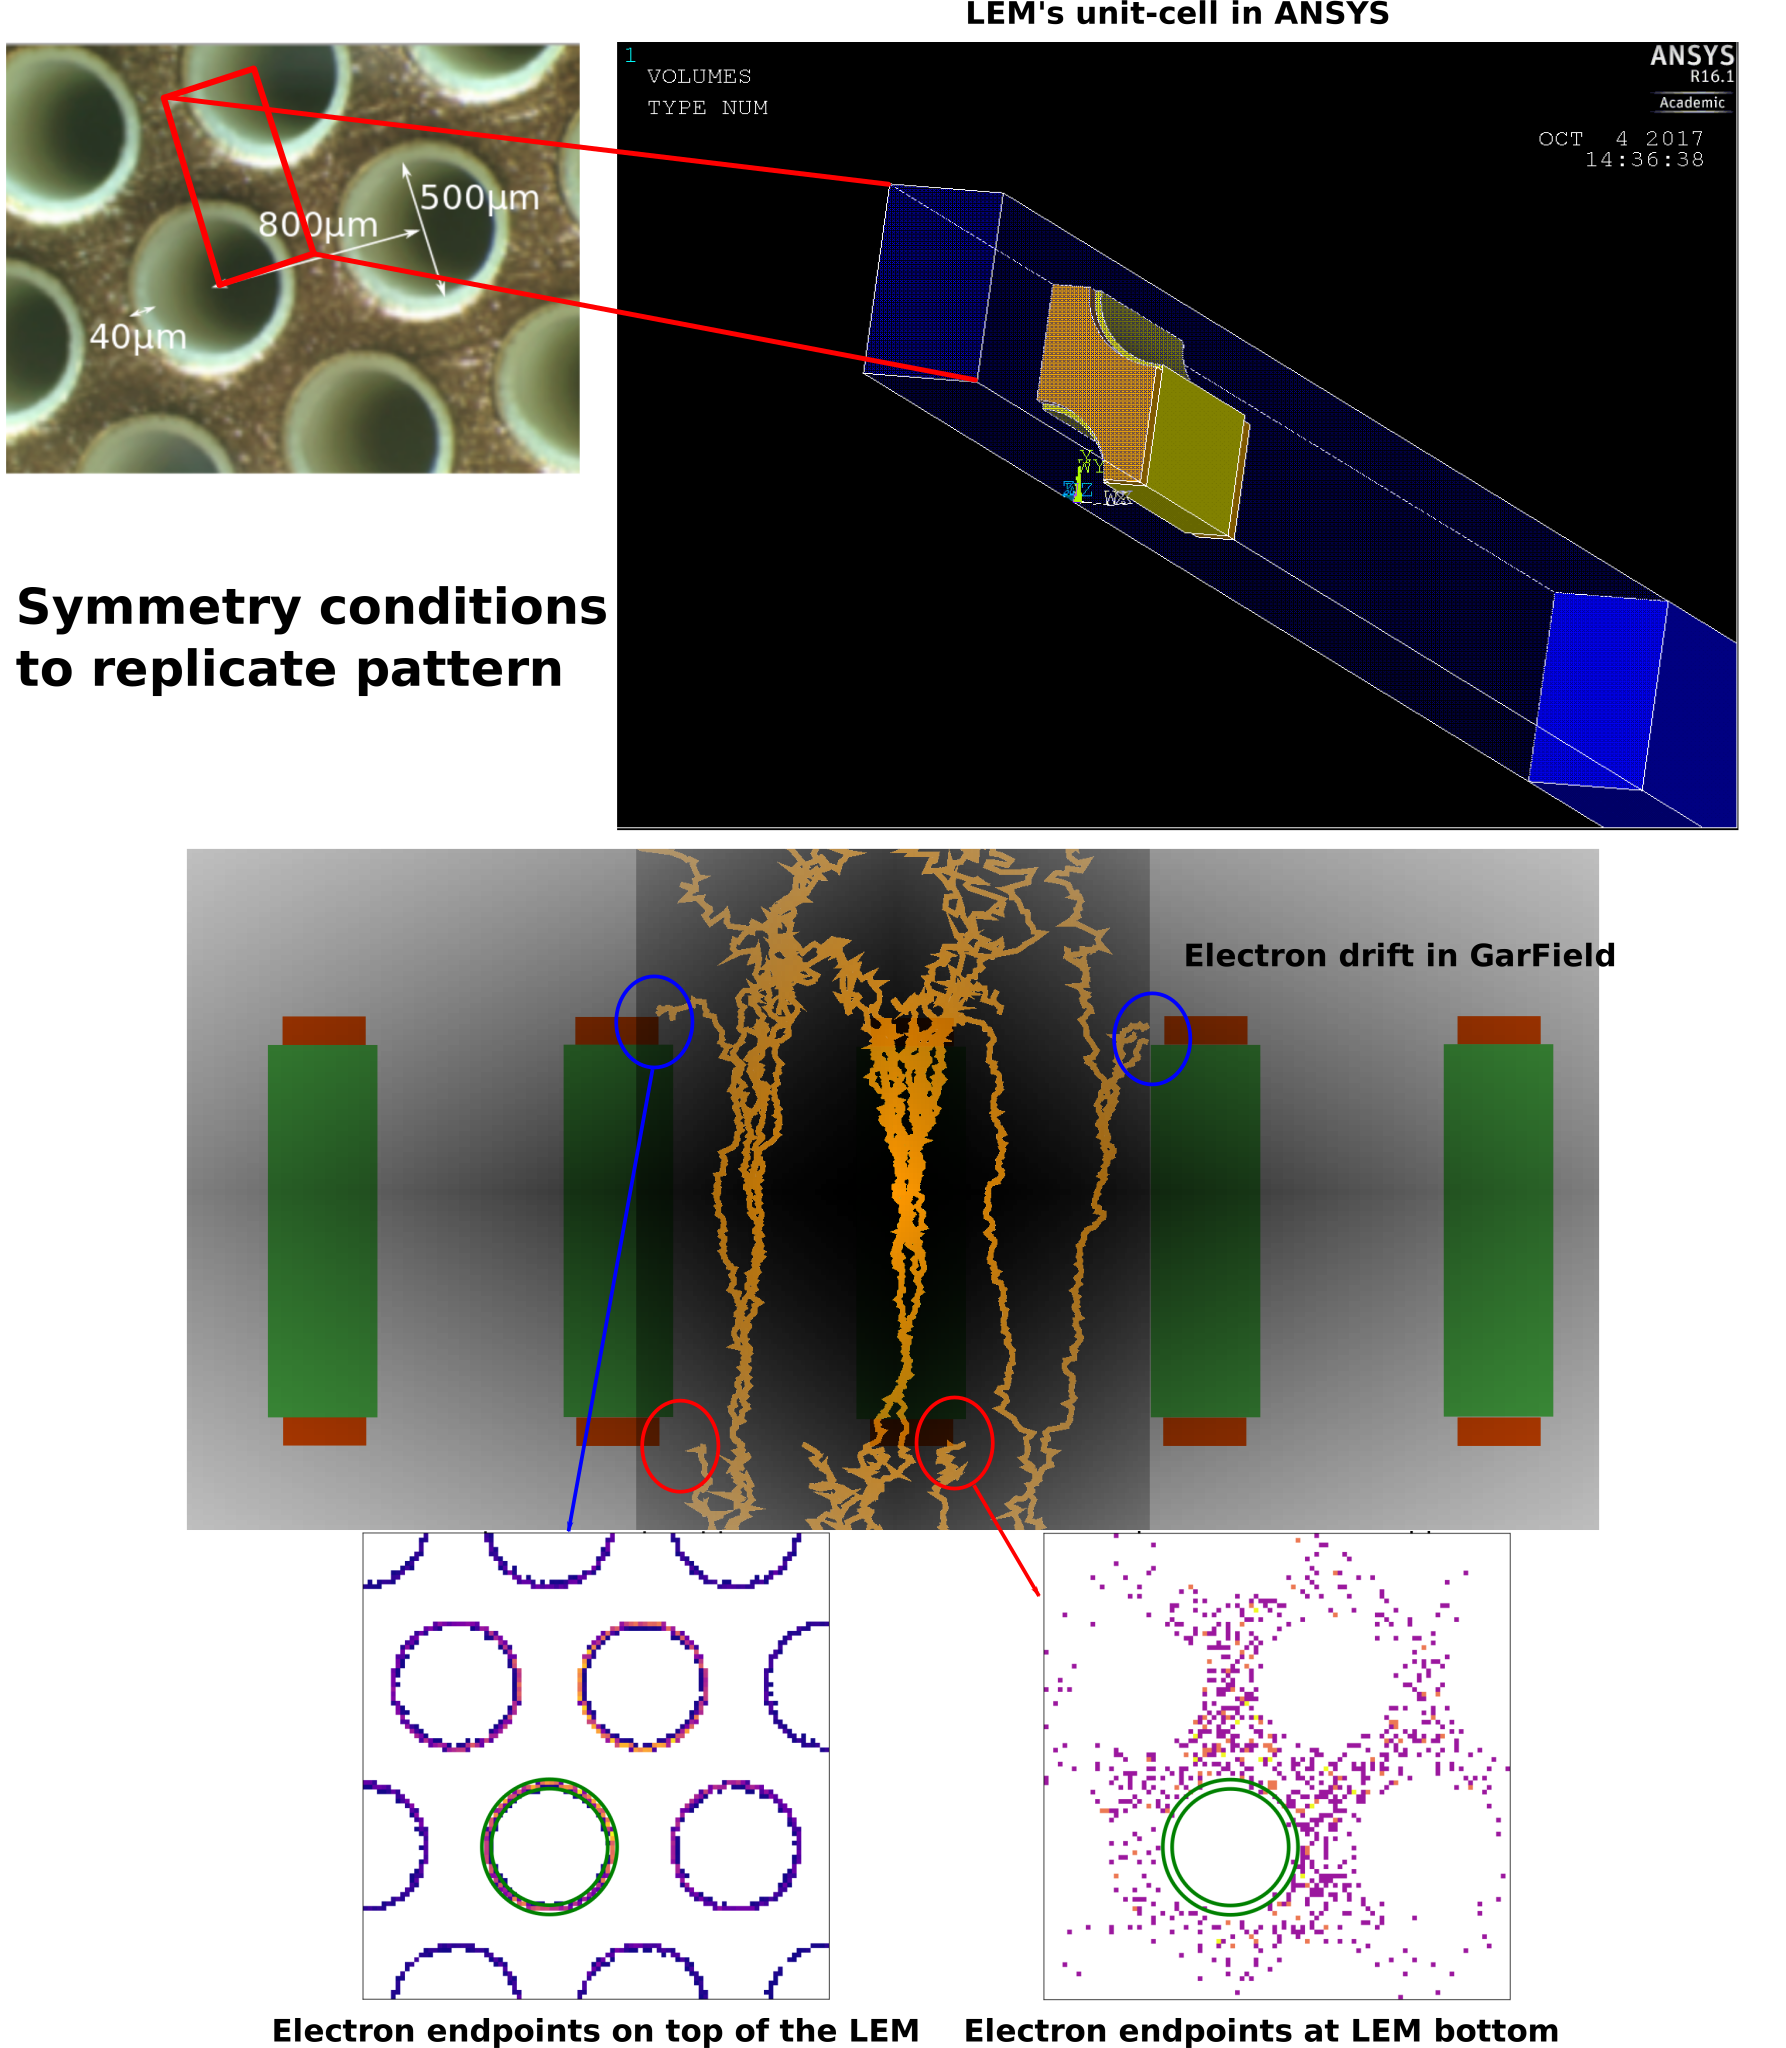
\includegraphics[width=\textwidth]{figures/311/coll_proba.png}\\
    		\end{minipage}\\
    		\vspace{0.2cm}
    		$\textcolor{red}{\text{LEM coll. Proba}}=\text{(Entering hole)}/\text{(initially generated)} \Rightarrow$ Influenced by \textbf{extraction} and \textbf{amplification} fields. \\
    		$\textcolor{blue}{\text{Anode coll. Proba}}=\text{(Reaching anode)}/\text{(Entering hole + amplified - lost in LEM)}\Rightarrow$ Influenced by \textbf{induction} and \textbf{amplification} fields.
    	\end{scriptsize} 
    \end{frame}
    
    \begin{frame}{The \texorpdfstring{$3 \times 1 \times \SI{1}{\meter\cubed}$}{311} prototype}{Study of extraction and induction fields effect on collected charge}
    	\begin{scriptsize}
    		\centering \includegraphics[width=\textwidth]{figures/311/effs.png}\\
    	\end{scriptsize} 
    \end{frame}
    
%    \begin{frame}{The \texorpdfstring{$3 \times 1 \times \SI{1}{\meter\cubed}$}{311}
%    		\begin{scriptsize}
%    		\end{scriptsize} prototype}{Purity and electron lifetime}
%    	Plots and fit
%    \end{frame}

% extrapolating charging up : 
%     tau(t) seems linear with a slope of -0.21 days/kV/cm
%     tau(33) = 0.54 -> tau(28) = 0.54+5*0.21 ~ 1.6
%     G0/Ginf = 2.7 independant of field
%     G(t) = (G0/2.7)/(1-(1-1/2.7)*exp(-t/tau)
				  %= G0/(2.7-(2.7-1)*exp(-t/tau)))
%    G(t)/G0 = 1/(2.7-(2.7-1)*exp(-t/tau))
%    G(t)/G0 = 1/(2.7-1.7*exp(-t/tau))
%     6h = 0.25 days
%    G(0.25)/G0 = 1/(2.7-1.7*exp(-0.25/1.6)) = 0.8
    
    \begin{frame}{The \texorpdfstring{$3 \times 1 \times \SI{1}{\meter\cubed}$}{311} prototype}{Gain vs amplification}
    	\begin{scriptsize}
	    	\begin{columns}
	    		\begin{column}{0.5\textwidth}
	    			\centering
	    			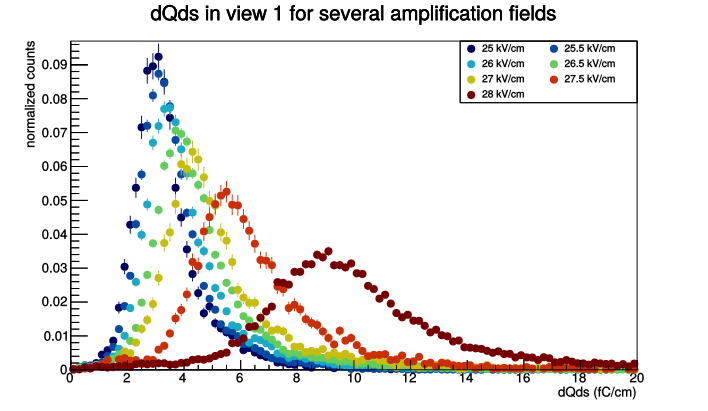
\includegraphics[width=\textwidth]{figures/311/dQds_gain.png}\\
	    			\vfill
	    			\begin{itemize}
	    				\item[$\bullet$] Use expected MPV of cosmic muons of \SI{7.75}{\femto\coulomb\per\centi\meter} to compute effective gain.
	    				\item[$\bullet$] Use simulated collection probabilities to compute equivalent gain at 3L fields (Induction of \SI{5}{\kilo\volt\per\centi\meter} and Extraction of \SI{2}{\kilo\volt\per\centi\meter} in liquid).
	    				\item[$\bullet$] Use the ratio $G_{3L}/G_{311}$ to study gain vs data taking time.
	    			\end{itemize}
	    		\end{column}
	    		\hfill
	    		\begin{column}{0.5\textwidth}
	    			\centering
	    			\includegraphics[width=.9025\textwidth]{figures/311/gain.png}\\
	    			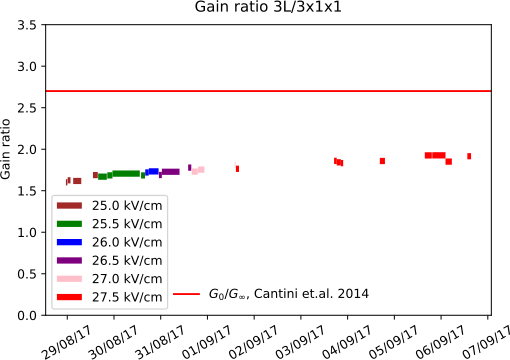
\includegraphics[width=.95\textwidth]{figures/311/ratio_vs_time.png}\\
	    		\end{column}
	    	\end{columns}
	    	$\Rightarrow G_{311} \simeq G_{3L}/1.5$. No clear explanation.\\
	    	$\Rightarrow$ Indication for persistent charging up.\\
    	\end{scriptsize}
    \end{frame}
    
    \begin{frame}{The \texorpdfstring{$3 \times 1 \times \SI{1}{\meter\cubed}$}{311} prototype}{Gain vs amplification : Higher Amplification fields}
    	\begin{scriptsize}
    		\centering
    		\includegraphics[width=0.9\textwidth]{figures/311/bad_track.png}\\
    		\vfill
    		\begin{columns}
    			\begin{column}{0.5\textwidth}
    				\begin{itemize}
    					\item[$\bullet$] Grid voltage limited\\ $\Rightarrow$ Higer amplification means lower extraction.
    					\item[$\bullet$] \textcolor{red}{Charge reconstruction fails : \\MPV(view 0)$\sim5\times$MPV(view 1)}\\(should be $\sim$equal).
    				\end{itemize}
    			\end{column}
    			\hfill
    			\begin{column}{0.5\textwidth}
    				\begin{itemize}
    					\item[$\bullet$] Developed a dedicated reconstruction software.
    					\item[$\bullet$] Better noise removal for better charge reconstruction.
    					\item[$\bullet$] Still under construction.
    				\end{itemize}
    			\end{column}
    		\end{columns}
    	\end{scriptsize}
    \end{frame}
    
    \begin{frame}{The \texorpdfstring{$3 \times 1 \times \SI{1}{\meter\cubed}$}{311} prototype}{Gain vs amplification : Higher Amplification fields}
    	\begin{scriptsize}
    		\centering
    		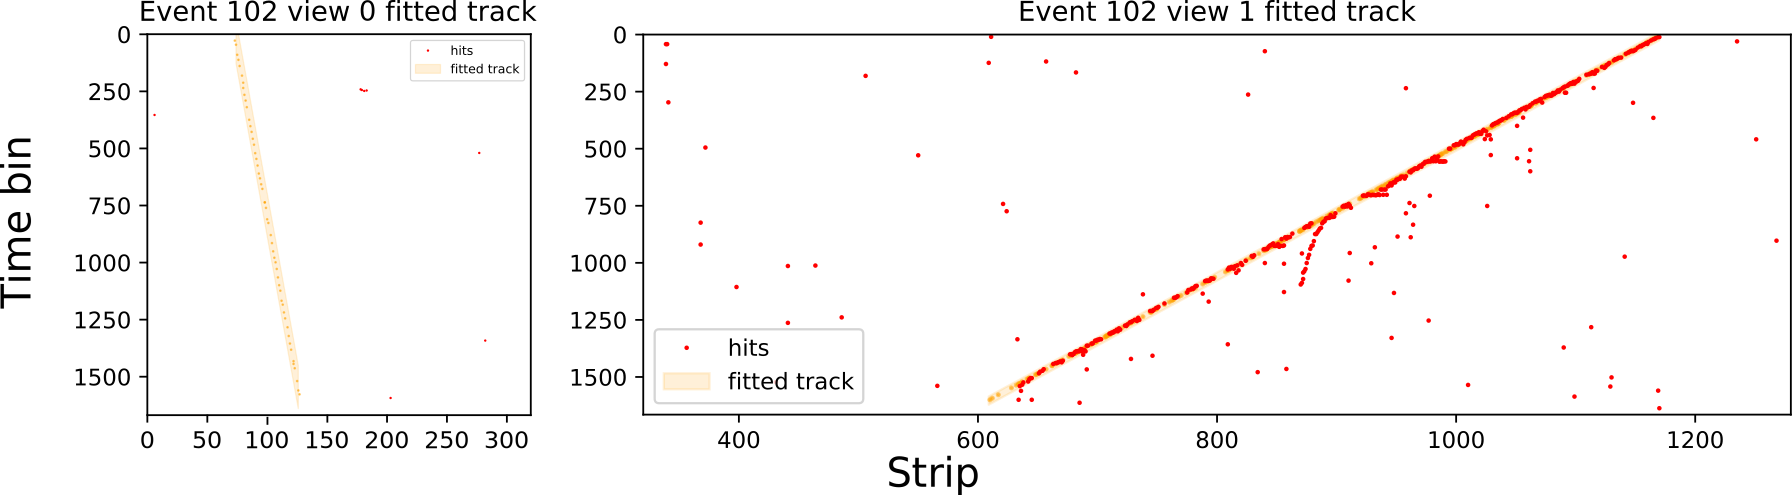
\includegraphics[width=0.9\textwidth]{figures/311/rawdatasoft_track.png}\\
    		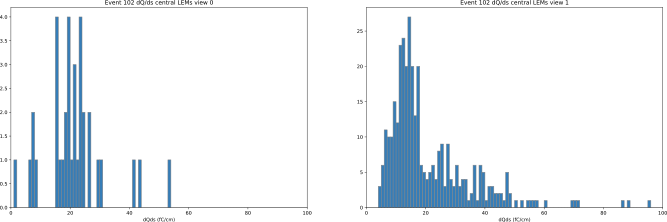
\includegraphics[width=0.9\textwidth]{figures/311/rawdatasoft_dQds.png}\\
    		\vfill
    		\begin{columns}
    			\begin{column}{0.5\textwidth}
    				\begin{itemize}
    					\item[$\bullet$] MPV(view 0)$\sim5\times$MPV(view 1).
    					\item[$\bullet$] But MPV(view 0) a bit lower.
    				\end{itemize}
    			\end{column}
    			\hfill
    			\begin{column}{0.5\textwidth}
    				\begin{itemize}
    					\item[$\bullet$] Will compare to well reconstructed tracks.
    					\item[$\bullet$] \textbf{Shortcoming} : very slow. Will process only a few tracks per amplification field.
    				\end{itemize}
    			\end{column}
    		\end{columns}
    	\end{scriptsize}
    \end{frame}
    
    \begin{frame}{Conclusion}
    	\begin{itemize}
    		\item[$\bullet$] $3 \times 1 \times \SI{1}{\meter\cubed}$ proved DLArTPC technology with large readout area and \si{\meter\cubed} volume.
    		\item[$\bullet$] It pointed out problems that are being solved in the $6 \times 6 \times \SI{6}{\meter\cubed}$.
    		\item[$\bullet$] Data taking with the $6 \times 6 \times \SI{6}{\meter\cubed}$ should begin this summer.
    	\end{itemize}
    \end{frame}
    
\end{document}

